% --------------------------------------------------
% 
% This chapter is for HPC
% 
% --------------------------------------------------

\chapter{
   An overview of the computational requirements \& solutions in microbial ecology
}
\label{cha:hpc}

\section[0s and 1s in marine molecular research: a regional HPC perspective]{
   0s and 1s in marine molecular research: a regional HPC perspective\footnote{
      For author contributions, please refer to the relevant section. Modified version of the published review.
   } 
}

\textbf{Citation:}
Zafeiropoulos, H., Gioti, A., Ninidakis, S., Potirakis, A., Paragkamian, S., ... \& 
Pafilis, E. (2021). 0s and 1s in marine molecular research: a regional HPC perspective. 
GigaScience, 10(8), giab053, doi: \href{https://doi.org/10.1093/gigascience/giab053}{10.1093/gigascience/giab053}


% ZORBA ABSTRACT
   \subsection{Abstract}
   High-performance computing (HPC) systems have become indispensable for modern marine research, 
   providing support to an increasing number and diversity of users. Pairing with the impetus 
   offered by high-throughput methods to key areas such as non-model organism studies, their 
   operation continuously evolves to meet the corresponding computational challenges. 

   Here, we present a Tier 2 (regional) HPC facility, operating for over a decade at the 
   Institute of Marine Biology, Biotechnology, and Aquaculture of the Hellenic Centre for Marine Research in Greece. 
   Strategic choices made in design and upgrades aimed to strike a balance between depth 
   (the need for a few high-memory nodes) and breadth (a number of slimmer nodes), as dictated by the 
   idiosyncrasy of the supported research. 
   Qualitative computational requirement analysis of the latter revealed the diversity of marine fields, 
   methods, and approaches adopted to translate data into knowledge. 
   In addition, hardware and software architectures, usage statistics, policy, and user management aspects 
   of the facility are presented. Drawing upon the last decade's experience from the different levels of operation 
   of the Institute of Marine Biology, Biotechnology, and Aquaculture HPC facility, a number of lessons are presented; 
   these have contributed to the facility's future directions in light of emerging distribution technologies (e.g., containers) 
   and Research Infrastructure evolution. 
   In combination with detailed knowledge of the facility usage and its upcoming upgrade, 
   future collaborations in marine research and beyond are envisioned.


   % ZORBA INTRODUCTION
   \subsection{Introduction}

   The ubiquitous marine environments (more than 70\% of the global surface \citep{noaa}) 
   mold Earth's conditions to a great extent. 
   The interconnected abiotic \citep{falkowski2008microbial} and biotic factors 
   (from bacteria \citep{falkowski2008microbial} to megafauna \citep{estes2016megafaunal}), 
   shape biogeochemical cycles \citep{arrigo2005marine} and climates \citep{boero2007conceptual, beal2011role} 
   from local to global scales. 
   In addition, marine systems have high socio-economic value \citep{remoundou2009valuation} 
   as an essential source of food and by supporting renewable energy and transport, 
   among other services \citep{portner2019ocean}. 
   The study of marine environments involves a series of disciplines (scientific fields): 
   from Biodiversity \citep{sala2006global} and Oceanography to (eco)systems biology \citep{tonon2015marine} 
   and from Biotechnology \citep{dionisi2012bioprospection} to Aquaculture \citep{tidwell2001fish}.

   To shed light on the evolutionary history of (commercially important) 
   marine species \citep{carvalho1995molecular}, as well as on how invasive species respond and 
   adapt to novel environments \citep{sakai2001population}, 
   the analysis of their genetic stock structure is fundamental \citep{begg1999holistic}. 
   Similarly, biodiversity assessment is essential to elucidate ecosystem functioning \citep{loreau2000biodiversity} 
   and to identify taxa with potential for bioprospecting applications \citep{leal2012trends}. 
   Furthermore, systems biology approaches provide both theoretical and technical backgrounds 
   in which integrative analyses flourish \citep{norberg2001phenotypic}. 
   However, conventional methods do not offer the information needed to explore the 
   aforementioned scientific topics.
   
   High-throughput sequencing (HTS) and sister methods have launched a new era in many 
   biological disciplines \citep{mardis2008next, kulski2016next}. 
   These technologies allowed access to the genetic, transcript, protein, and metabolite 
   repertoire \citep{goodwin2016coming} of studied taxa or populations, and facilitated the analysis of 
   organism-environment interactions in communities and ecosystems \citep{bundy2009environmental}. 
   Whole-genome sequencing and whole-transcriptome sequencing approaches provide valuable 
   information for the study of non-model taxa \citep{cahais2012reference}. 
   This information can be further enriched by genotyping-by-sequencing approaches, 
   such as restriction site-associated DNA sequencing \citep{baird2008rapid}, or by investigating gene 
   expression dynamics through Differential Expression (DE) analyses \citep{tarazona2011differential}. 
   Moving from single species to assemblages, molecular-based identification and functional 
   profiling of communities has become available through marker (metabarcoding), 
   genome (metagenomics), or transcriptome (metatranscriptomics) sequencing from environmental 
   samples \citep{goldford2018emergent}. 
   To a great extent, these methods address the problem of how to produce and get access 
   to the information on different biological systems and molecules.

   These $0$s and $1$s of information (i.e., the data) come along with challenges regarding their 
   management, analysis, and integration \citep{merelli2014managing}. 
   The computational requirements for these tasks exceed the capacity of a standard laptop/desktop by far, 
   owing to the sheer volume of the data and to the computational complexity of the bioinformatic algorithms 
   employed for their analysis. 
   For example, building the de novo genome assembly of a non-model Eukaryote may require algorithms 
   of nondeterministic polynomial time complexity. 
   This analysis can reach up to several hundreds or thousands of GB of memory (RAM) \citep{sohn2018present}. 
   Hence, the challenges of how to exploit all these data and how to transform data into knowledge set 
   the present framework in biological research \citep{greene2014big, pal2020big}.
   
   To address these computational challenges, the use of high-performance computing (HPC) systems 
   has become essential in life sciences and systems biology \citep{lampa2013lessons}. 
   HPC is the scientific field that aims at the optimal incorporation of technology, methodology, 
   and the application thereof to achieve “the greatest computing capability possible at any point 
   in time and technology" \citep{sterling2017high}. 
   Such systems range from a small number to several thousands of interconnected computers (compute nodes). 
   According to the Partnership for Advanced Computing in Europe, the European HPC facilities are categorized as: 
   (i) European Centres (Tier 0), 
   (ii) national centers (Tier 1), and 
   (iii) regional centers (Tier 2) [33] \citep{enwiki:1009652575}. 
   As the Partnership for Advanced Computing in Europe highlights, "computing drives science and science drives computing" 
   in a great range of scientific fields, from the endeavor to maintain a sustainable Earth to efforts to expand 
   the frontiers in our understanding of the universe \citep{lindahl2018scientific}. 
   On top of the heavy computational requirements, biological analyses come with a series of other practical issues 
   that often affect the bioinformatics-oriented HPC systems.

   Researchers with purely biological backgrounds often lack the coding skills or even the 
   familiarity required for working with Command Line Interfaces \citep{lindahl2018scientific}. 
   Virtual Research Environments are web-based e-service platforms that are particularly useful 
   for researchers lacking expertise and/or computing resources \citep{candela2013virtual}. 
   Another common issue is that most analyses include a great number of steps, with the software 
   used in each of these having equally numerous dependencies. A lack of continuous support 
   for tools with different dependencies, as well as frequent and non-periodical versioning of the latter, 
   often results in broken links and further compromises the reproducibility of analyses [36]. 
   Widely used containerization technologies—e.g., Docker \citep{rad2017introduction} and Singularity \citep{kurtzer2017singularity}—ensure reproducibility 
   of software and replication of the analysis, thus partially addressing these challenges. 
   By encapsulating software code along with all its corresponding dependencies in such containers, 
   software packages become reproducible in any operating system in an easy-to-download-and-install 
   fashion, on any infrastructure.

   The \href{https://imbbc.hcmr.gr/}{Institute of Marine Biology Biotechnology and Aqua-culture (IMBBC)} 
   has been developing a computing hub that, in conjunction with national and European Research Infrastructures (RIs), 
   can support state-of-the-art marine research. 
   The regional IMBBC HPC facility allows processing of data that derive from the Institute's sequencing platforms 
   and expeditions and from multiple external sources in the context of interdisciplinary studies. 
   Here, we present insights from a thorough analysis of the research supported by the facility and some 
   of its latest usage statistics in terms of resource requirements, computational methods, and data types; 
   the above have contributed in shaping the facility along its lifespan.


   % ZORBA CONTRIBUTION
   \subsection{Contribution}

   % ZORBA METHODS
   \subsection{Methods}

   \subsubsection*{The IMBBC HPC Facility: From a Single Server to a Tier 2 System}

   





% ZORBA RESULTS
\subsection{Results}



\begin{figure}[h]
   \centering
   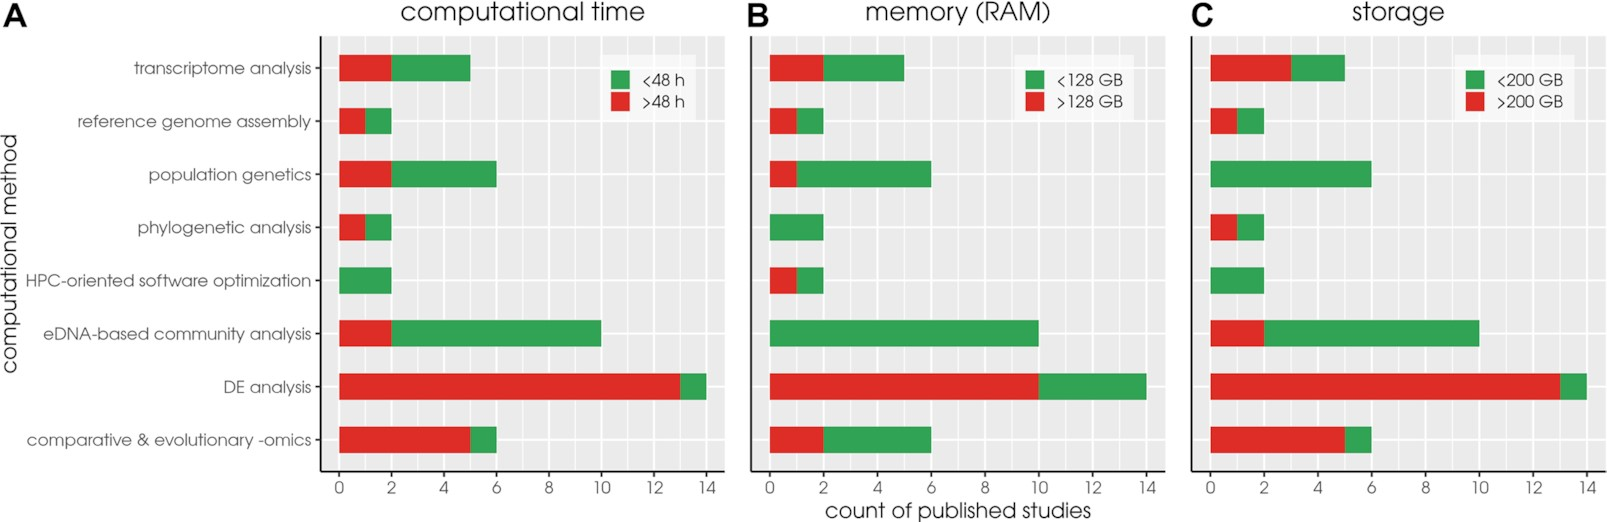
\includegraphics[width=140mm]{figures/zorbas_jobs_resources.jpeg}
   \caption{Computing requirements of the published studies performed on the IMBBC HPC facility over the last decade. Figure from publication.
   % Red bars denote published research with high resource requirements of the various computational methods employed at the IMBBC HPC facility due to (a) long computational times (>48 h), (b) high memory requirements (>128 GB), or (c) high storage requirements (>200 GB). For instance, no eDNA-based community analyses performed at Zorba thus far have required a large amounts of memory.
   }
   \label{fig:zorba_jobs}
\end{figure}


% ZORBA DISCUSSION
\subsection{Discussion}







